\documentclass[journal,twoside,web]{ieeecolor}
\usepackage{jsen}
\usepackage{cite}
\usepackage{amsmath,amssymb,amsfonts}
\usepackage{algorithmic}
\usepackage{graphicx}
\usepackage{caption}
\usepackage{textcomp}
\usepackage{wrapfig}
\usepackage{anyfontsize}
\usepackage{makecell}
\def\BibTeX{{\rm B\kern-.05em{\sc i\kern-.025em b}\kern-.08em
    T\kern-.1667em\lower.7ex\hbox{E}\kern-.125emX}}
\markboth{Spring 2020}
{Author \MakeLowercase{\textit{et al.}}: Preparation of Papers for IEEE TRANSACTIONS and JOURNALS (February 2020)}
\begin{document}
\title{Ireland Temperature Data Analytics}
\author{Ranjith Pozhiparambil Ravindran
\thanks{Under the supervision of Dr. Shagufta Henna, Letterkenny Institute of Technology, Letterkenny, CO. Donegal }
}

\IEEEtitleabstractindextext{
\begin{abstract}
In This project we analyze Ireland earth surface temperature data since 1900 to derive insights on impact on global warming in Ireland.  Goal of this analysis is to understand the rate of temperature change in Ireland since 1900 and decades where it is at its peak, predict yearly average temperature for future years and compare temperature change over seasons since 1900.  The data set is quite huge and contain data of all the countries since 1740.  Apache Spark with Hadoop File System (HDFS) is used to store, filter and analysis this data.  Jupyter Notebook interface is used for code development in pyspark.  Polynomial regression machine learning model is used to understand trend of earth surface temperature increase in Ireland and project temperature of Ireland in future years.   As part of this project, we also analyze increase in temperature across seasons with the objective of understanding whether the winter season is getting more or less colder. Python matplotlib library is used to visualization of these analyses.
\end{abstract}

\begin{IEEEkeywords}
Big Data Analysis, Spark mlib, Spark ML Generalized linear regression, spark dataframe, Spark SQL
\end{IEEEkeywords}}

\maketitle

\section{Introduction}
\label{sec:introduction}
\IEEEPARstart{G}{lobal} warming has been a major concern all over the world for a while. In last 30 years, we could see a rapid growth in average earth surface temperature. Global warming has impact on temperature and whether of Ireland as the winter season is getting milder and summer is becoming warmer.  Average temperature of Ireland has increased 0.8 degree Fahrenheit in last two decades \cite{I1}. This change is in all levels, both land and ocean temperature change almost mirror one another.  Industrial revolution has been major contributor for the temperature change since 1900 and the population growth rate increase started around 1975(from 2.5 billion in 1950 to 5 billion in 2000) had made impact on global warming much bigger.   Global warming is defined as the increase in extreme temperature and measuring it in terms of average yearly temperature may not be accurate.  Even though the average yearly temperature change might not be very evident, there are more days with extreme temperature.  So, as part of this project, we are trying to take average extreme temperature by considering only the temperature reading in summer season (May to October).  In this project we analyze Ireland earth surface temperature data since 1900 to derive insights on impact on global warming in Ireland.  The source data is huge and contain monthly temperature reading of all cities since 1970, so it will be stored and processing in Hadoop Distributed File System (HDFS).  Jupyter Notebook interface with Pyspark is used for the development of the project and spark SQL is used for aggregation of data for analysis.  Visualization of result is done using python learning libraries matplot and numpy.  Polynomial regression algorithm  was used to build machine learning model to visualize rate of temperature change and predict future temperature.  Spark ML library and Python numpy library is available to develop polynomial regression machine learning modes.  We have developed ML model using both these libraries and compared them to get more accurate result.  Spark ML data pipeline feature is used in this project to build spark ML model in this project.  Code and other files related to this project is uploaded to github (https://github.com/ranjithpr1984/IrelandTemperatureDynamics).

\section{Data description}
World earth surface temperature dataset from Kaggle\cite{DATA} is used as source data for this project.  The dataset has 5 CSV files with average monthly temperature for all the countries and cities across the world, but only file "GlobalLandTemperaturesByCity.csv" was used.  Below are the fields in file "GlobalLandTemperaturesByCity.csv".

\begin{enumerate}
\item dt :- Month in date format with date as 1st
\item AverageTemperature :-  Average earth surface temperature in Celsius for a month and city
\item City name
\item Country name 
\item Latitude of the city
\item Latitude of the city
\end{enumerate}

\section{Related works}
The data for this project is sourced from Kaggle and the dataset has many linked projects in Kaggle with variety of analyses and visualizations. Most of them are focused on visualizing the impact of global warming across the world, also these projects are aggregating the temperature of whole year for their analysis \cite{RW}.  In this project, we focus on analyzing the impact of global warming in Ireland.  Global warming is defined as the increase in extreme temperature, so unlike other current projects, this project focus on analyzing the temperature on summer temperature instead of whole year.  This ensure that extreme temperature in summer season is not reversed by extreme cold in winter season.

\section{System architecture}
This project was built on hadoop cluster of three nodes build using virtual machines (VM) and data analysis and visualization is done in Jupyter Notebook using pyspark.  Figure \ref{SA} shows architecture of the system which contain four layers.  The bottom layer is hadoop cluster with hadoop file system.  Hadoop cluster contains three nodes, built using VMs with CentOS 7.  Hadoop cluster was chosen for this project to distribute the storage and processing of large source file.  Spark master and slaves are running on hadoop cluster to use pyspark for analysis and visualization.  Distributed data analytics jobs can be easily developed using spark dataframe and Pyspark SQL, which avoid the need for developing complex map reduce programs.  Jupyter Notebook interface is used to develop and run pyspark code.  Jupyter Notebook is very user friendly interface for development, debugging and testing code and very widely used in Big data analytics.

\begin{figure}[h]
\centering
\captionsetup{justification=centering}
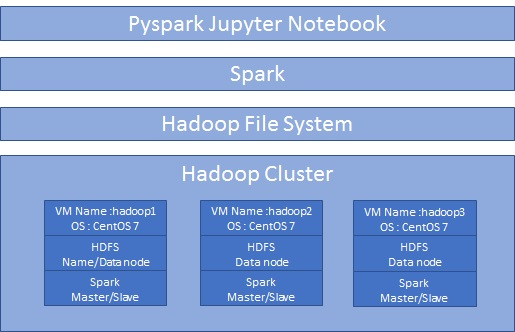
\includegraphics[scale=.65]{System_architecture.jpg}
\caption{System architecture}
\label{SA}
\end{figure}

\section{Ireland Temperature Prediction}
As discussed in the introduction, one of the objectives of this project is to understand the trend of temperature increase in Ireland and predict temperature for future years.  In the data set we have data till 2013 and we will try to predict Ireland temperature till 2040.  Machine Learning (ML) model was developed and trained using polynomial regression algorithm for this prediction.  There were two options for developing polynomial regression machine learning model and they are Spark ML Generalized linear regression and python one dimensional polynomial regression.  Both these options were explored because of their advantages and disadvantages.  Spark ML Generalized linear regression support multidimensional features and does distributed machine learning which helps in fast train on large distributed data sets, but it required more coding to prepare data in the form required by the spark ML library. Python poly1d model support only one feature, but it is easy to implement and very fast on small data sets. Figure \ref{ITPDPL} shows the data pipeline of Ireland temperature prediction and following subsections explain each stage in the pipeline.

\begin{figure}[h]
\centering
\captionsetup{justification=centering}
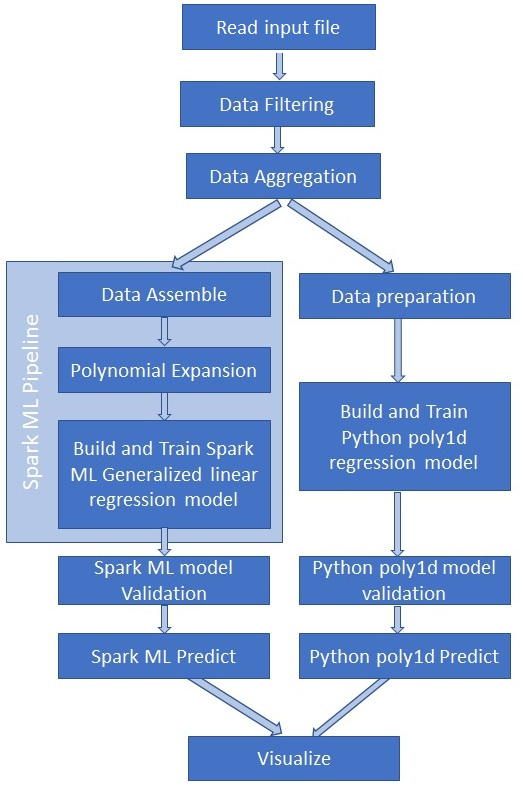
\includegraphics[scale=.55]{Ireland_Temperature_Prediction_Data_Pipeline.jpg}
\caption{Ireland Temperature Prediction Data Pipeline}
\label{ITPDPL}
\end{figure}

\subsection{Read input file}
First step in the data pipeline is to read the source CSV file into spark dataframe.  Pyspark provide API to read CSV and return dataframe.  This API also support inferring schema for spark dataframe from header row of the file with parameter "header". When using this feature to automatically build schema for spark dataframe, it should be kept in mind that the data type for all the columns will be set to string type, so required type casting should be done on the dataframe later.

\subsection{Data Filtering}
The source data contain temperature reading of all cities across the world since 1970 and it also contain many records with blank reading.  So, first data processing stage in the data pipeline is to filter only Ireland data since 1900 with valid temperature reading.  Also, the source data has total six columns, out of which we need only date and temperature data. So, as part of the filtering, only these columns are selected for next stage.  Standard python required long map reduce programs to implement this filtering, but using pyspark dataframe functions "select()" and "filter()", it can be implemented with single line of code.  Function "select()" is used fetch only date and temperature column and function "filter()" is used to filter data with country as Ireland, temperature reading not blank and date is greater than 1st january 1900.

\subsection{Data Aggregation}
Data filtering stage reduces large data set into small data set of around 1200.  This still is bit too much to plot in a graph and it is difficult to infer a polynomial function which can fit all these data points.  So, the dataset has to be further reduced by taking the average yearly temperature with 5 years window.  For example, the temperature since 1900-1905 will be aggregated into single record by taking average of these.  Like this average of temperature is taken for every five years, so that final data set contains around 20 records only.  Impact of global warming is extreme cold temperature in winter and extreme hot temperature in summer.  So, the average temperate of whole year may not show the change in extreme temperature because it might be balanced by extreme cold temperature in winter of the same year.  Because of this, while doing aggregation, we have considered only temperature readings for summer months (May-August) to derive average extreme temperature of the year.  Even if we use spark dataframe functions, computation of average temperature for every five year is bit complex task.  We have used Spark SQL feature to implement this complex computation with simple SQL statement.  Spark dataframe function "createOrReplaceTempView()" was used to create a temporary table on top of the filtered spark dataframe.  Function "spark.sql()" was used to run SQL query against the temporary table.  Spark SQL function executes SQL query against temporary table and returns the query result as dataframe.  Spark SQL helps developers to implement complex computations and filtering using standard SQLs which is much easier than programming and most of the analysts and developers are very familiar with SQL.  With this aggregation data is reduced to 20 records and it is ready for analysis.

\subsection{Data Assemble}
Spark ML libraries required training dataset in the form of labels and features and the features should be in single column with multi-dimensional array.  Spark transformer "VectorAssembler()" from Spark ML features was used to convert feature column into multi-dimensional array of features. 

\subsection{Polynomial Expansion}
Change of temperature in over last 100 years cannot be described using a straight linear regression line, because in last few decades there has been sharp increase compared to first half of the century.  We need to use polynomial regression to build machine learning model to predict future temperature.  Unfortunately, Spark ML doesn't have a specific API for polynomial regression, but we can simulate polynomial regression using spark features polynomial expansion and Generic linear regression APIs.  Polynomial expansion API help us to convert our single dimensional feature vector into higher dimension feature vector. We can then feed this high dimensional vector data to Spark ML Generalized Linear Regression with family "tweedie" to produce polynomial regression model.  In this project our dataframe was converted into 4-dimensional vector using polynomial expansion transformer to get polynomial regression curve with maximum accuracy.

\subsection{Build and Train Spark ML Generalized linear regression model}
Spark ML Generalized Linear Regression (GLR) is used to build and train polynomial regression model for predicting Ireland's average summer (April-August) temperature for future years.  Spark ML GLR was invoked with family as "tweedie" and linkPower as 4 to produce polynomial regression model.  Spark ML pipeline feature was used to build spark ML data pipeline to Assemble, poly expand, build and train ML model.

\subsection{Spark ML model validation}
Validation of model was done by feeding the same data used for training the model.  Then compare the actual temperature and predicted temperature using scikit learn to find R-square score.  R-square score Spark ML model is 0.7215321564144628.  We have also evaluate the model by plotting source data and regression curve on graph. Figure \ref{PRMV} shows the source data points in red color and Spark ML model regression curve in green color. We can see that the curve fits reasonably well across the data points. Python matplot library is used for ployting this graph.

\subsection{Spark ML Predict}
We trained spark ML model using source data of Ireland temperature till 2010 and using this model we have predicted Ireland's average summer(April-August) temperature for period of 2011-2040.  Green curve in figure \ref{IRSTP} shows the predicted average summer temperature for Ireland for period of 2011-2040.

\subsection{Data preparation}
Python polynomial regression model is light and fast for smaller dataset.  Since we have already reduced the size of the dataset by aggregation and we have only one feature (Year), we can also use Python one dimensional polynomial regression(poly1d) for this prediction.  Python poly1d requires label and feature in form of 2-dimensional array variables.  As part of data preparation step, we need to convert spark dataframe into array variables.  We have converted spark dataframe with aggregation result into python Panda dataframe and used values method of Panda dataframe to extract the columns into array variables. 

\subsection{Build and Train Python poly1d regression model}
Polynomial regression API "polyd()" from python library "numpy" was used to build the Polynomial regression model. Two 2-Dimensional arrays with year and temperature data from aggregated data was used to train the model.

\subsection{Python poly1d model validation}
We have fed year collection(array) used for training to model, and the model has returned collection(array) of predicted temperature for those years.  Then compared the actual temperature and predicted temperature using scikit learn to find R-square score.  R-square score Python poly1d model is 0.730108027223213.  We can see that accuracy of Python poly1d regression model is slightly higher than Spark ML model.  We have also plotted the regression curve of the model in figure \ref{PRMV} with a blue curve. 

\subsection{Python poly1d Predict}
A collection(array) of year values 2010-2040 was passed to python polynomial regression model and it returned collection(array) with corresponding predicted temperature.  Green curve in figure \ref{IRSTP} shows average summer temperature for Ireland for period of 2011-2040, predicted using python poly1d model.

\subsection{Visualization}
Figure \ref{PRMV} shows data points and polynomial regression curve of the models build using spark ML and python numpy library.        Regression curve of both models are plotted in same figure for easy comparison. We can see regression curve of both models are almost similar and fit most of the data points.  From regression curve, it is very evident that there has been sharp rise in temperature in last 3 decades (since 1980).  Even though the regression curve of both models are almost same, this sharp increase in temperature in last 30 years were interpreted slightly different by these two models.  This difference is very evident in figure \ref{IRSTP}, temperature increase predicted by Python polyd model is slightly higher than spark ML model.  Spark ML predicts average summer temperate is expected to reach around 17.1 by 2040, where Python poly1d model predict it will reach 19.8.  We could collected average summer temperate data for last three years (2017-2019) from Ireland whether site MET eireann.  Table \ref{table} shows the comparison of Met eireann reading with prediction of both models.  In this comparison, we could see that even though python poly1d model had more accuracy with training data, prediction of spark ML model is more closer actual temperature of period 2017-2019.

\begin{table}
\centering
\caption{Comparison of prediction with Met eireann data}
\label{table}
\fontsize{9}{10.5}\selectfont
\begin{tabular}{|l|l|l|l|}
\hline
Year & Met eireann & Spark ML & Python poly1d\\
\hline
2017 & 14.90 & 14.99 & 15.33 \\
\hline
2018 & 16.05 & 15.07 & 15.45 \\
\hline
2019 & 15.05 & 15.14 & 15.57 \\
\hline
\end{tabular}
\label{tab1}
\end{table}

\begin{figure}[h]
\centering
\captionsetup{justification=centering}
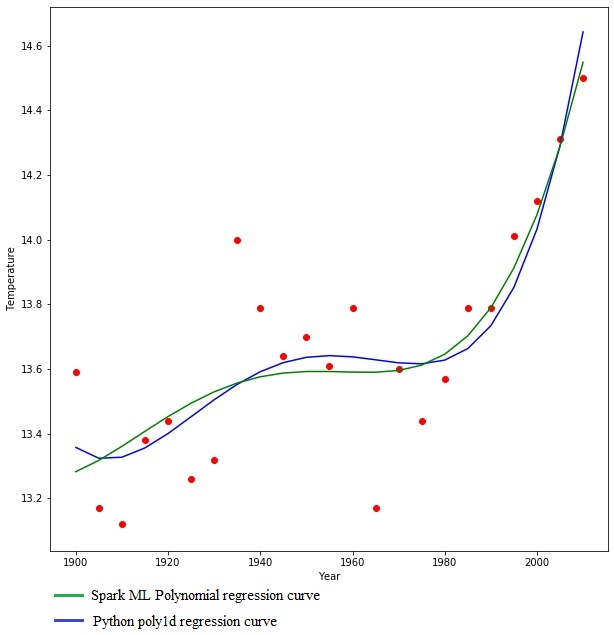
\includegraphics[scale=.50]{Poly_model_validation.jpg}
\caption{Polynomial regression model validation}
\label{PRMV}
\end{figure}

\begin{figure}[h]
\centering
\captionsetup{justification=centering}
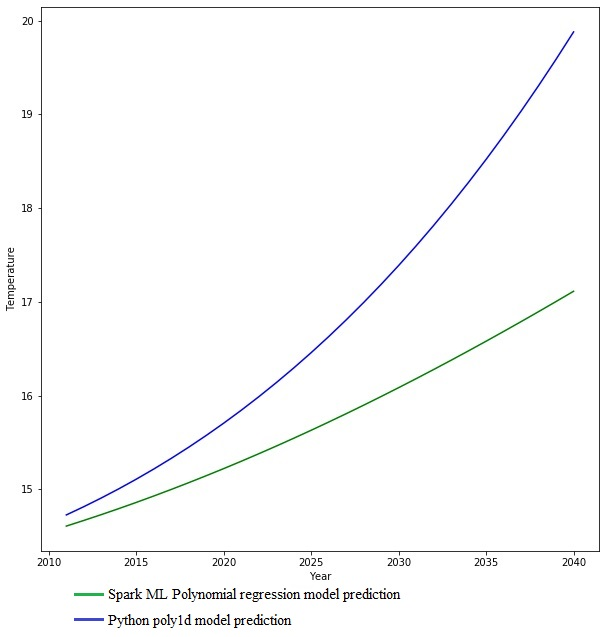
\includegraphics[scale=.50]{Ireland_future_summer_temperature_prediction.jpg}
\caption{Ireland future summer temperature prediction}
\label{IRSTP}
\end{figure}

\section{Ireland Seasonal Temperature Analysis}
Impact of global warming is ideally extreme cold weather in winter and extreme hot weather in summer. In this project we had also analyzed whether this is true for Ireland. We have aggregated average monthly temperature of Ireland for each decade and plotted it in graph using python matplot library.  Figure \ref{ISTADP} shows the data pipeline of Ireland seasonal temperature analysis. First 2 stages in the data pipeline is same as data pipeline of Ireland temperature prediction analysis and only last 3 stages are explained in following subsections.

\begin{figure}[h]
\centering
\captionsetup{justification=centering}
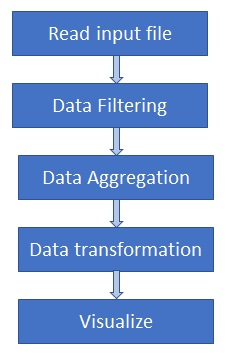
\includegraphics[scale=.50]{Ireland_Seasonal_Temperature_Analysis_Pipeline.jpg}
\caption{Ireland Seasonal Temperature Analysis data pipeline}
\label{ISTADP}
\end{figure}

\subsection{Data aggregation}
For seasonal temperature analysis we have aggregated monthly temperature data for every 10 year. For example, January temperature data of year 1900-1910 is aggregate into one record.  The aggregated result has 12 records (1 per month) for every 10 years and resulting spark dataframe has around 120 records with three columns year, month and temperature.  Spark SQL was used for this aggregation and SQL was executed against spark temporary table created during temperature prediction analysis.

\subsection{Data transformation}
To easily plot the data, month and temperature field in aggregated spark dataframe was pivoted into collections(array). The resulting dataframe has only 10 records (1 per every 10 year) and each records has fields months and temperature which are collections with data for 12 months of that year.  This transformation was achieved using spark dataframe aggregation and collection features.

\subsection{Visualization}
Ireland temperature data since 1900, across year is plotted in figure \ref{ISTA}.  X-axis represent months and Y-axis represent temperature.  We can see temperature distribution across year is a curve with low values in winter months and reaches its peak on July.  Figure has 10 curves in unique colors representing average temperature distribution across year for each decade, since 1900. Starting decades are represented with shades of blue, mid decades are represent with shades of purple and ending decades are represented with shades of red. Curves with red shade represent last 3 decades and we can see that winter temperature of last 30 years is higher compared to winter temperature of earlier decades.  And obliviously summer temperature is increasing which we also saw in our earlier analysis.  Based on this analysis, we can see that for Ireland, since last 30 years winter is getting less colder and summer is getting more hotter.

\begin{figure}[h]
\centering
\captionsetup{justification=centering}
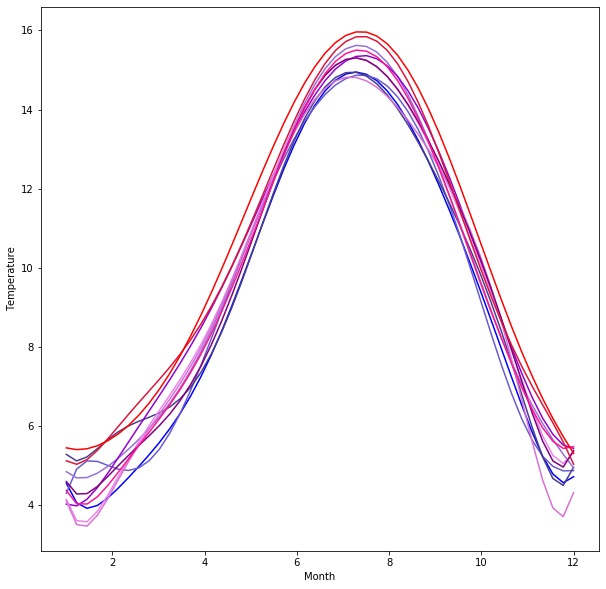
\includegraphics[scale=.50]{Ireland_Seasonal_Temperature_Analysis.jpg}
\caption{Ireland Seasonal Temperature Analysis}
\label{ISTA}
\end{figure}

\section{Conclusion}
As part of this project, we have done two types of data analysis on Ireland temperature data between 1900 and 2010. First analysis was to understand the trend of temperature change in last century and try to predict temperature for future years.  Based on our analysis and visualization results, we could see that there has been a sharp rise in summer temperature during last 30 years.  Increase in summer temperature for first 80 years of the century (1900-1980) was just 0.5 degree Celsius(13.6 - 13.1). But in last 30 years (1980-2010) the temperature has increased by 1.1 degree Celsius, which is double compared to 80 years before that.  If this trend continues, it will reach around 16-17 degree Celsius in 2030 and 17-20 degree Celsius in 2040.  We also found that even though the general trend of global warming impact across the globe is extreme cold winter and extreme hot summer, but when it comes to Ireland winter is getting less colder and summer is getting more hotter.  To conclude, it is evident that temperature is increasing and in last few decades the rate of increase is very high compared to earlier decades. Increase in earth surface temperature is caused by increase in emissions of greenhouse gases in the atmosphere which is cause by increase in  production. In last few decades there has been an increase in production due to the increase in machine automation and foreign trading. A sharp increase in population growth rate started around 1975 has also resulted in increase in production.  Impact of this increase is earth surface temperature is more frequent hurricanes and heat waves, devastating droughts and wildfires. Last year Irish Wildlife Trust (IWT) has recorded 15 wildfires from counties Cork, Kerry, Waterford, Galway, Donegal, Louth and Mayo. Mankind must act on it before it is too late and implement necessary remedies to reduce emissions of greenhouse gases to keep this sharp increase in temperature under control. 

\begin{thebibliography}{00}
\bibitem{I1} Edward J Markey, \emph{EnergyIndependanceAndGlobalWarming} [Online]. Available: \underline{https://www.markey.senate.gov/GlobalWarming/impactzones/ireland.html}

\bibitem{DATA} kaggle, \emph{kaggle} [Online]. Available: \underline{https://www.kaggle.com/berkeleyearth/climate-change-earth-surface-temperature-data}

\bibitem{RW} kaggle, \emph{kaggle} [Online]. Available: \underline{https://www.kaggle.com/berkeleyearth/climate-change-earth-surface-temperature-data/kernels}

\bibitem{METEIREANN} MET eireann, \emph{METeireann} [Online]. Available: \underline{https://www.met.ie/climate/available-data/monthly-data}


\end{thebibliography}


\end{document}
